\chapter{Results}

\section{Theoretical results}
\subsection{Interference}

We now formally define a notion of interference between subsets. 

\begin{definition}
    (\textbf{\textit{k}-Interference}) Given two sets $U, W$, and some number $k \in (0,|W|]$, we say $U$ $k-$\textit{interferes} with $W$ if 
    \begin{equation}
        |U \cap W| \ge  \frac{|W|}{k}.
    \end{equation}
\end{definition}

\begin{corollary}
    \label{collorary:k-int-equals}
        If $|U| = |W|$, then $U$ $k$-interferes with $W$ if and only if $W$ $k$-interferes with $U$.
    \end{corollary}
    
We restrict the upper range of $k$ to $|W|$ for convenience, as beyond that all values of $\frac{|W|}{k}$ will be less than 1.

This is a generalization of the notion of interference introduced by Valiant in 2005. Valiant defines a memory to be in a ``firing" state if more than half the nodes in the memory are in a ``firing" state. He then defines interference as the unintential firing of a memory $W$ when another memory $U$ is fired, which is possible if and only if more than half the nodes of $W$ are also present in $U$ \cite{valiant2005memorization}. This corresponds to the $k = 2$ case of our definition. 

We are now interested in finding the probability of a randomly picked subset interfering with another randomly picked subset. We start with the case where they are randomly picked as we believe it is the simplest case. We will touch upon other possible cases in the Discussion section below when discussing models in Computational Neuroscience that use unique memory generation algorithms.

\begin{lemma}
    \label{lemma:k-int-prob}
	Given a set $V$ with $n$ items and two subsets $U,W$ of respective sizes $r_u,r_w$, denote the size of the intersection between them by the random variable $Y$. Then the probability of $U$ $k$-interfering with $W$ is $$\sum_{y = \left\lceil \frac{r_w}{k} \right\rceil}^{r_w} \frac{\binom{r_u}{y} \binom{n-r_u}{r_w-y}}{\binom{n}{r_w}}$$ and $Y \sim Hypergeometric(n, r_u, r_w)$.
\end{lemma}
\begin{proof}
	If $V = \{v_1,...,v_n\}$, we can represent the first randomly picked subset $U$ as a boolean vector $u$ of length $n$ defined by
    $$
    u_i = \begin{cases}
        1 & \text{if } v_i \in U \\
        0 & \text{if } v_i \notin U.
    \end{cases}
    $$
    With this representation, $U$ will intersect another randomly picked subset $W$ at the indices where both boolean vectors $u, w$ have a $1$. Then $Y$ denotes the number of indices where both $u, w$ have a 1. First note that
    \begin{equation}
        \mathbb{P}(Y=y) = \frac{\binom{r_u}{y} \binom{n-r_u}{r_w-y}}{\binom{n}{r_w}}.
    \end{equation}
    This follows from the fact that given the first vector $U$, we already know where the 1's are located. We can pick the $y$ intersecting 1's for the second vector in $\binom{r_u}{y}$ ways implicitly placing 0's in the remaining spots. We then fill the remaining $n-r_u$ indices corresponding to the 0's in the first vector with $r_w-y$ 1's in $\binom{n-r_u}{r_w-y}$ ways. Finally we divide by the total number of possible subsets $\binom{n}{r_w}$. Clearly, this is the probability mass function of the hypergeometric distribution with population size $n$, $r_u$ success states and $r_w$ draws. We conclude that $Y \sim Hypergeometric(n, r_u, r_w)$. Finally, to find the probability of $U$ $k$-interfering with $W$ we need to find $\mathbb{P}(Y \ge \left\lceil \frac{r_w}{k} \right\rceil)$ which is the sum of $\mathbb{P}(Y=y)$ from $y = \left\lceil \frac{r_w}{k} \right\rceil$ to $y = r_w$.
\end{proof}

For brevity, we can reinterpret the above probability as the tail distribution function of $Y$ at $\left\lfloor \frac{r_w}{k} \right\rfloor$, 
$$
\mathbb{P}\left(Y \geq \left\lceil \frac{r_w}{k} \right\rceil\right) = \mathbb{P}\left(Y > \left\lfloor \frac{r_w}{k} \right\rfloor\right) = \bar{F}_Y\left(\left\lfloor \frac{r_w}{k} \right\rfloor\right)
$$
Recall from statistics that the expectation of a binary payoff, like intersection, that depends on a cutoff (in this case $\left\lceil \frac{r_w}{k} \right\rceil$) is equal to the probability of the variable being greater than or equal to the cutoff. Therefore the probability in lemma \ref{lemma:k-int-prob} is equal to the expected number of interferences of $U$ with $W$. 

We then want to estimate the expected number of interferences when the sizes of the subsets are within a certain offset of $r$, say $\delta$ without being exactly equal to $r$. This approach will make our results more applicable to models like the Neuroidal Model that assume memory sizes follow some distribution \cite{valiant2005memorization}. The offset can be selected to best suit the distribution involved. For example if the sizes come from a discrete distribution like $\mathcal{B}(r/p,p)$, and if the variance $r(1-p)$ is more than $10$, it makes sense to choose $\delta  = 2\sqrt{r(1-p)}$ since roughly 95\% of all values lie within $[r-2\sigma,r+2\sigma]$.

Generalizing this without any further assumptions is quite hard as the binomial coefficients do not vary nicely as a function of two variables over their domain. Instead we will make a reasonable assumption that will allow us to derive a reasonable lower bound for this expectation in terms of a general parameter instead of individual subset sizes. 

\begin{lemma}
    \label{lemma:expected-k-int-prob}
    Given a set $V$ with $n$ items and two subsets $U,W$ of respective sizes $r_u,r_w$, denote the size of the intersection between them by the random variable $Y$.
        If \begin{enumerate}
            \item $r_u, r_w \in [r-\delta, r+\delta]$ for some $r, \delta > 0$,
            \item $n >> 2(r+\delta)$, 
        \end{enumerate}      
then $$ \bar{F}_Y\left(\left\lfloor \frac{r_w}{k} 
\right\rfloor\right) \ge \sum_{y = \left\lceil \frac{r+\delta}{k} \right\rceil}^{\left\lfloor r - \delta \right\rfloor} \frac{\binom{r-\delta}{y} \binom{n-r-\delta}{r-\delta-y}}{\binom{n}{r+\delta}}$$
    \end{lemma}
    \textit{Remark.} Before proceeding with the proof, we want to justify the second assumption made here. It is a known fact that bounding binomial coefficients above or below is hard due to the nature of how it varies with respect to the second argument. We know that $n \choose k$ reaches its maximum value at $\left\lceil \frac{n}{2} \right\rceil$ or $\left\lfloor \frac{n}{2} \right\rfloor$ and it is monotonically increasing at smaller values and decreasing at larger values. My making the assumption here we can ensure that our second argument is always a lot smaller than this maxima, and as such an increase in the second argument will only increase the value of the expression. This assumption is reasonable since models like the Neuroidal Model expect the memory sizes to be significantly smaller than the size of the model \cite{valiant2005memorization}. Also note that the binomial coefficient increases monotonically with respect to the first argument. 
    \begin{proof}  
        First note that $n > r_u, r_w$ and by extension $n > r$ since the size of a subset cannot exceed the size of the set.  
        Then observe that 
        \begin{equation}
            \begin{split}
                \bar{F}_Y\left(\left\lfloor \frac{r_w}{k} \right\rfloor\right)  
                &=
                 \sum_{y = \left\lceil \frac{r_w}{k} \right\rceil}^{r_w} \mathbb{P}(Y=y)  
                \\[2em] &=    \sum_{y = \left\lceil \frac{r_w}{k} \right\rceil}^{r_w} \frac{\binom{r_u}{y} \binom{n-r_u}{r_w-y}}{\binom{n}{r_w}} 
                \\[2em] &\ge  \sum_{y = \left\lceil \frac{r_w}{k} \right\rceil}^{r_w} \frac{\binom{r-\delta}{y} \binom{n-r-\delta}{r-\delta-y}}{\binom{n}{r+\delta}}  
                \\[2em] &\ge  \sum_{y = \left\lceil \frac{r+\delta}{k} \right\rceil}^{\left\lfloor r - \delta \right\rfloor} \frac{\binom{r-\delta}{y} \binom{n-r-\delta}{r-\delta-y}}{\binom{n}{r+\delta}}  
            \end{split}
        \end{equation}
        The first and second equalities follow from the definition of the tail distribution and lemma \ref{lemma:k-int-prob} respectively. The third inequality follows from assumption 1. in the theorem and the behavior of the binomial coefficient under varying arguments. The final inequality follows from the fact that since all terms in the sum are positive, reducing the number of terms will make the overall expression smaller.
        
    \end{proof}

    \subsection{Capacity}
    With the above lemmas in our arsenal we can now move on  the main subject of this thesis. We now formally define the capacity of a system of overlapping subsets with interference being the limiting factor. 

    \begin{definition} (\textbf{(\textit{$r,T,k,\delta$})-Subset Capacity}) Given a set $V = \{v_1,...,v_n\}$, and parameters $r, T, k, \delta > 0$, the \textit{$(r,T,k,\delta)$-subset capacity} of $V$ is the \textit{maximum} number of subsets that can be picked subject to the conditions that for any randomly picked subset $U$,
        \begin{enumerate}
            \item $|U| \in [r-\delta,r+\delta]$,
            \item $n >> 2(r+\delta)$,
            \item \label{equ:cap-bound-expected}$E[X_U] \le T$ where $X_U$ is a random variable denoting the number of interferences caused due to picking $U$. 
        \end{enumerate}
    \end{definition}

    We need the second restriction on the memories here since we want to apply lemma \ref{lemma:expected-k-int-prob} to every pair. The third restriction here can be thought of as a stopping criteria as we stop picking the subsets once the expectation of interference reaches that threshold. In the context of models in computational neuroscience like the Neuroidal Model, this means that there will be too much impact on the quality of memorization, that is too much noise and misfiring in the system if we add any further memories.
    
    Before deriving the capacity for the general case, let us consider the simpler case where all memories have the exact same size. This is valuable since it results in a much simpler expression and we can use this as an approximation for the more general case too. However note that we realize this scenario is not biologically plausible at all. 

    \begin{theorem}
        \label{thm:exact-r}
        Given a set $V$ with $n$ items and the property that every picked subset will have size exactly $r$, the $(r,T,k,\delta)$-subset capacity of $V$ is 
        \begin{equation*}
            \left\lfloor \frac{T}{\bar{F}_Y\left(\left\lfloor \frac{r}{k} \right\rfloor\right)} + 1 \right\rfloor.
        \end{equation*}
    \end{theorem}

    \textit{Remark.} Since all subsets have fixed size $r$, note that the choice of $\delta$ is not relevant here.

    \begin{proof}[Proof 1.]
         Suppose we have already have $M-1$ subsets in the universe. Pick a random subset $U$. From lemma \ref{lemma:k-int-prob}, we know that the expected number of $k$-interferences of $U$  with another arbitrary subset $W$ from the universe is $\bar{F}_Y\left(\left\lfloor \frac{r}{k} \right\rfloor\right)$. Since there are $M-1$ other subsets, the total expected number of $k$-interferences caused by picking $U$ is $(M-1) \bar{F}_Y\left(\left\lfloor \frac{r}{k} \right\rfloor\right)$.

        From inequality \ref{equ:cap-bound-expected} in the definition of capacity, we have 
        
            \begin{equation}
            \label{equ:cap-exact-r}
                (M-1) \bar{F}_Y\left(\left\lfloor \frac{r}{k} \right\rfloor\right) \le T \implies M \le \frac{T}{\bar{F}_Y\left(\left\lfloor \frac{r}{k} \right\rfloor\right)} + 1.
            \end{equation}
            The $(r,T,k,\delta)$-subset capacity of $V$ then is the largest integer $M$ that satisfies inequality \ref{equ:cap-exact-r}.
    \end{proof}

    We provide an alternate proof that, while less elegant, can be scaled to prove the general statement. 

    \begin{proof}[Proof 2.]
        Suppose we have already have $M$ subsets in the universe. Pick two subsets $U,W$ without replacement. From lemma \ref{lemma:k-int-prob}, we know that the expected number of $k$-interferences of $U$ with $W$ is $\bar{F}_Y\left(\left\lfloor \frac{r}{k} \right\rfloor\right)$. Since we know all subsets have the same size, the expected number of $k$-interferences of $W$ with $U$ is the same. So the expected number of interferences caused by one pair is
    $$
    2\bar{F}_Y\left(\left\lfloor \frac{r}{k} \right\rfloor\right).
    $$
    We know that there are $\binom{M}{2} = M(M-1)/2$ such pairs so the expected number of total interferences is
    $$
    2 \cdot \frac{M(M-1)}{2} \bar{F}_Y\left(\left\lfloor \frac{r}{k} \right\rfloor\right)  =  M(M-1) \bar{F}_Y\left(\left\lfloor \frac{r}{k} \right\rfloor\right). 
    $$
    Since there are $M$ subsets, the expected number of interferences by choosing picking one subset is
    $$
    \frac{M(M-1)}{M} \bar{F}_Y\left(\left\lfloor \frac{r}{k} \right\rfloor\right))  = (M-1) \bar{F}_Y\left(\left\lfloor \frac{r}{k} \right\rfloor\right).
    $$
    From inequality \ref{equ:cap-bound-expected}, we have 

    \begin{equation}
        \label{equ:cap-exact-r-2}
        (M-1) \bar{F}_Y\left(\left\lfloor \frac{r}{k} \right\rfloor\right) \le T \implies M \le \frac{T}{\bar{F}_Y\left(\left\lfloor \frac{r}{k} \right\rfloor\right)} + 1.
    \end{equation}
The $(r,T,k,\delta)$-subset capacity of $V$ is the largest integer $M$ that satisfies inequality \ref{equ:cap-exact-r-2}.
    \end{proof}

We will now tackle the general case using the same strategy as above. 

\begin{theorem}
    Given a set $V$ with $n$ items, the $(r,T,k,\delta)$-subset capacity of $V$ is bounded above by
    \begin{equation*}
     \frac{T}{\sum_{y = \left\lceil \frac{r+\delta}{k} \right\rceil}^{\left\lfloor r - \delta \right\rfloor} \frac{\binom{r-\delta}{y} \binom{n-r-\delta}{r-\delta-y}}{\binom{n}{r+\delta}}} + 1
    \end{equation*}
\end{theorem}

\textit{Remark.} Note that we can only say it is bounded above and not the exact capacity as defined since we have to use lemma \ref{lemma:expected-k-int-prob}. However as $\delta \to 0$, this expression converges to the expression in theorem \ref{thm:exact-r}. 

\begin{proof}

    Suppose we have $M$ subsets $U_1,...,U_M$ with sizes $r_1,...,r_M$. Pick two subsets $U_i,U_j$. From lemma \ref{lemma:k-int-prob}, we know that the expected number of interferences caused by this pair is
    $$
    \bar{F}_Y\left(\left\lfloor \frac{r_j}{k} \right\rfloor\right) + \bar{F}_Y\left(\left\lfloor \frac{r_i}{k} \right\rfloor\right).
    $$
    We then sum over all possible pairings to get the expected number of total interferences:
    $$
    \sum_{(i,j) \in \Z\times\Z, 1 \le i,j \le M, i \ne j} \Biggl( \bar{F}_Y\left(\left\lfloor \frac{r_j}{k} \right\rfloor\right) + \bar{F}_Y\left(\left\lfloor \frac{r_i}{k} \right\rfloor\right) \Biggr).
    $$

\noindent Since there are $M$ subsets, the expected number of interferences by picking one subset is
    $$
    \frac{1}{M} \sum_{(i,j) \in \Z\times\Z, 1 \le i,j \le M, i \ne j}  \Biggl( \bar{F}_Y\left(\left\lfloor \frac{r_j}{k} \right\rfloor\right) + \bar{F}_Y\left(\left\lfloor \frac{r_i}{k} \right\rfloor\right) \Biggr).
    $$

\noindent From inequality \ref{equ:cap-bound-expected}, we have 

\begin{equation*}
      \frac{1}{M} \sum_{(i,j) \in \Z\times\Z, 1 \le i,j \le M, i \ne j}  \Biggl( \bar{F}_Y\left(\left\lfloor \frac{r_j}{k} \right\rfloor\right) + \bar{F}_Y\left(\left\lfloor \frac{r_i}{k} \right\rfloor\right) \Biggr)  \le T,
\end{equation*}
\noindent which implies
\begin{equation}
\label{equ:cap-r}      
       M \geq \frac{1}{T}\sum_{(i,j) \in \Z\times\Z, 1 \le i,j \le M, i \ne j}  \Biggl( \bar{F}_Y\left(\left\lfloor \frac{r_j}{k} \right\rfloor\right) + \bar{F}_Y\left(\left\lfloor \frac{r_i}{k} \right\rfloor\right)\Biggr). 
\end{equation}
Using lemma \ref{lemma:expected-k-int-prob} we get
\begin{equation}
\label{equ:cap-r-2}
    \begin{split}
           M &\ge
           \frac{1}{T}\sum_{(i,j) \in \Z\times\Z, 1 \le i,j \le M, i \ne j}  \Biggl( 2 \sum_{y = \left\lceil \frac{r+\delta}{k} \right\rceil}^{\left\lfloor r - \delta \right\rfloor} \frac{\binom{r-\delta}{y} \binom{n-r-\delta}{r-\delta-y}}{\binom{n}{r+\delta}}\Biggr) \\
           &=\frac{1}{T} \frac{M(M-1)}{2} \Biggl( 2 \sum_{y = \left\lceil \frac{r+\delta}{k} \right\rceil}^{\left\lfloor r - \delta \right\rfloor} \frac{\binom{r-\delta}{y} \binom{n-r-\delta}{r-\delta-y}}{\binom{n}{r+\delta}}\Biggr),
    \end{split}
    \end{equation} \\
\noindent which implies 
\begin{equation}
    \label{equ:cap-r-bounded}     
    M \le \frac{T}{\sum_{y = \left\lceil \frac{r+\delta}{k} \right\rceil}^{\left\lfloor r - \delta \right\rfloor} \frac{\binom{r-\delta}{y} \binom{n-r-\delta}{r-\delta-y}}{\binom{n}{r+\delta}}} + 1.
\end{equation}
The expected $(r,T,k,\delta)$-subset capacity of $V$ should be bounded above by this expression and the tightness of the bound will depend on the parameter $\delta$. 
\end{proof}

\section{Empirical results}

\subsection{Fixed subset size}
First we simulate the case for fixed subset size $r$. 

\begin{figure}%[h]
    \centering
    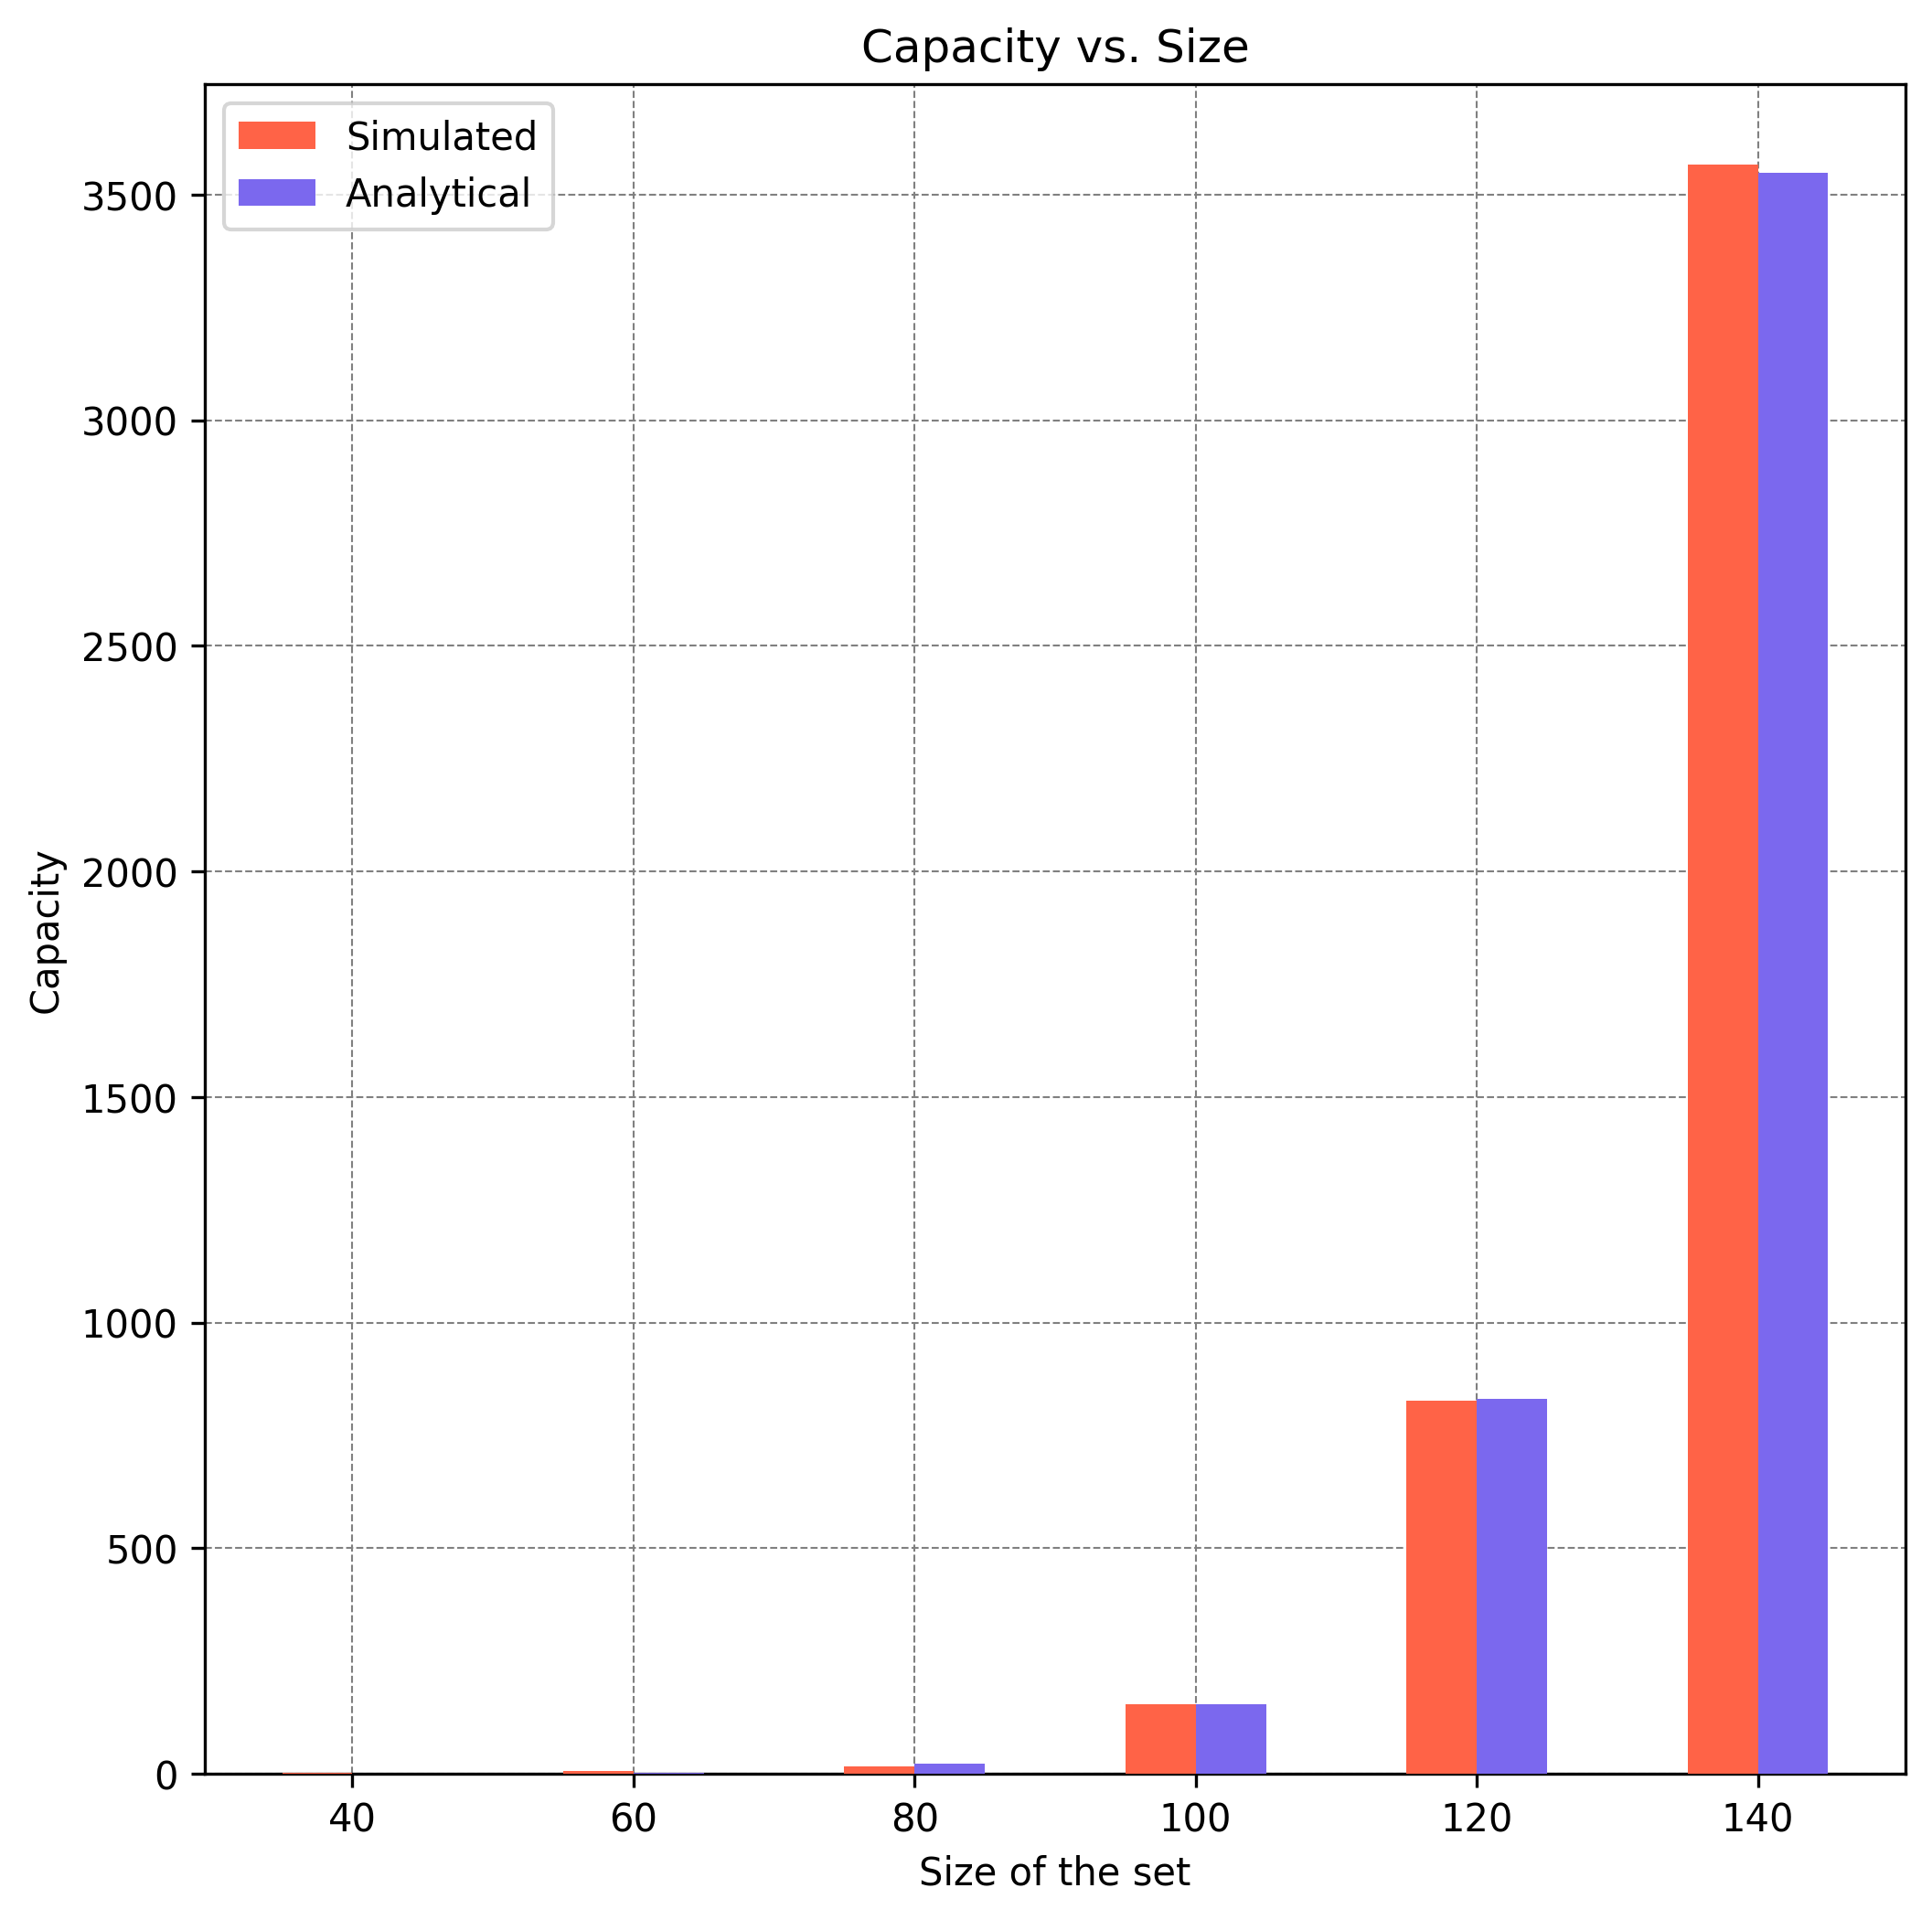
\includegraphics[scale=0.8]{figures/cap-vs-n.png}
    \caption[Capacity vs. Size of the set]{How capacity is affected by increasing the size of the set.}
    \label{figure:cap-vs-n}
    \end{figure}

We compare the average capacity of the simulation with the analytical result from Theorem \ref{thm:exact-r} as a function of the size of the set. We fix $r=20$, $k=2$, $T=0.1$. Figure \ref{figure:cap-vs-n} shows the results of this comparison. We see that the average simulated capacity is practically identical to the analytical capacity thoughout our input range.


    \begin{figure}%[h]
        \centering
        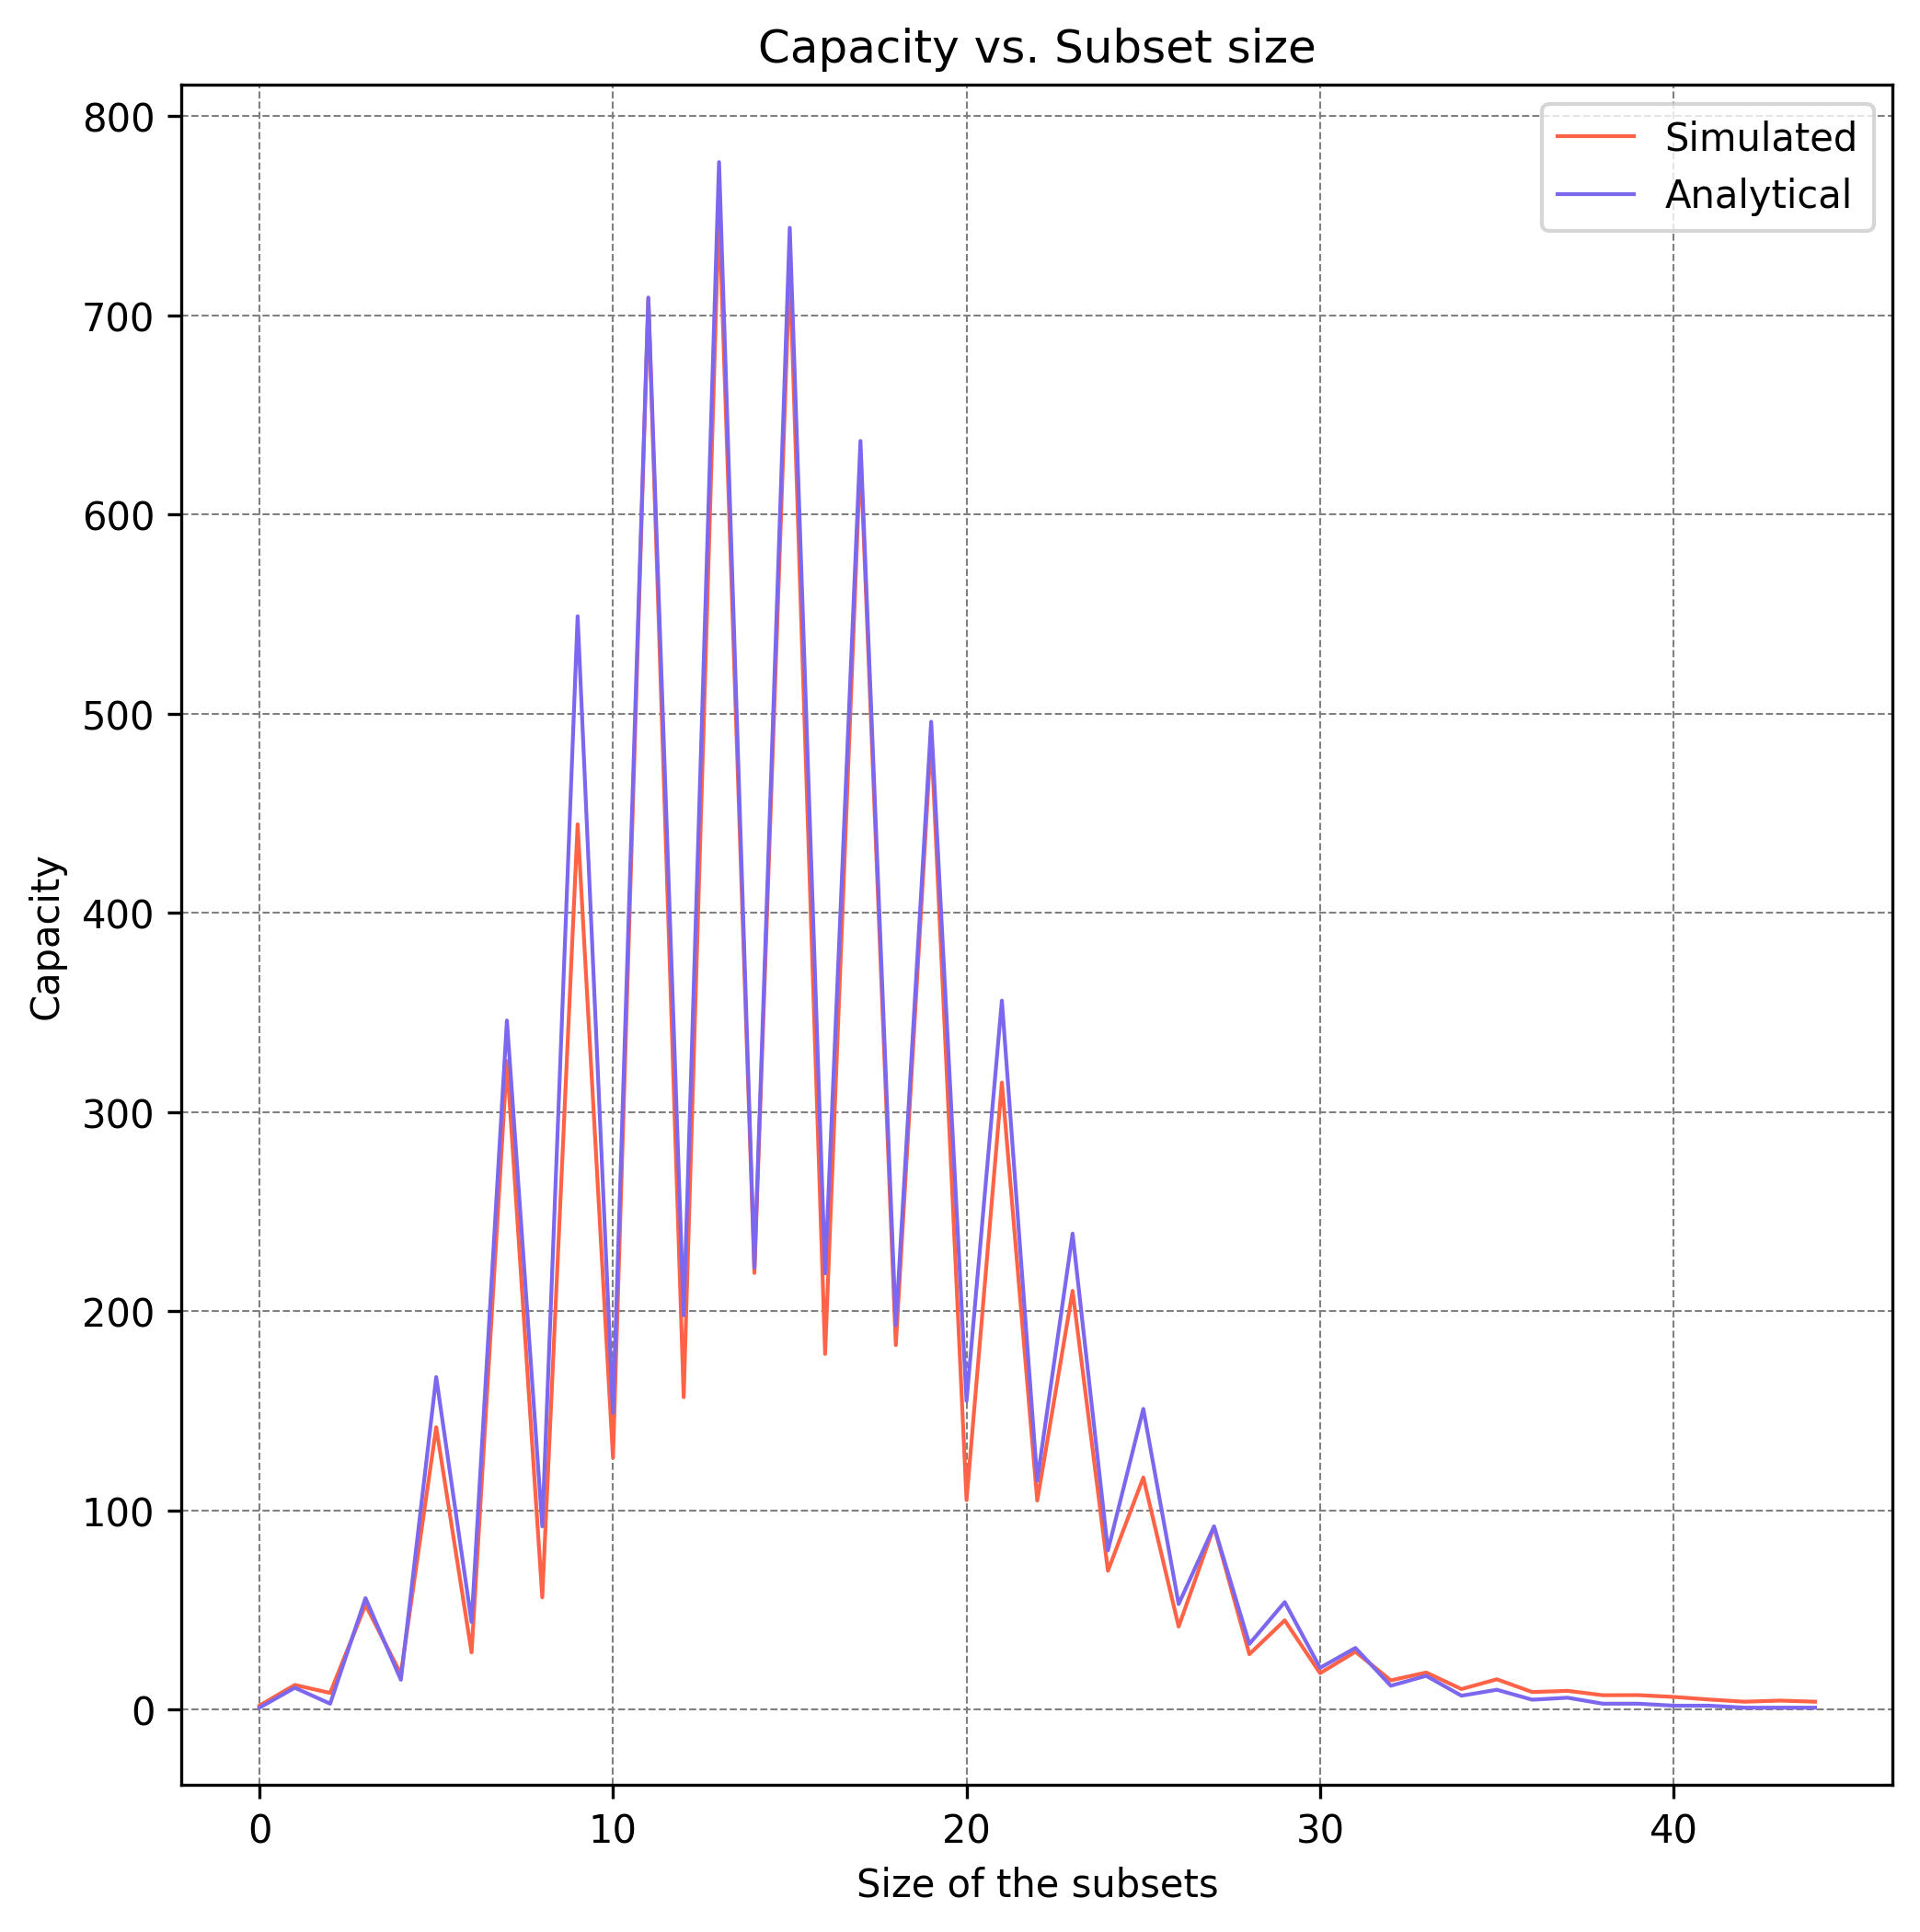
\includegraphics[scale=0.85]{figures/cap-vs-r.png}
        \caption[Capacity vs. Size of the subsets]{How capacity is affected by increasing the size of the subsets.}
        \label{figure:cap-vs-r}
        \end{figure}

Then we the compare the average capacity of the simulation with the analytical result from Theorem \ref{thm:exact-r} as a function of the size of the subsets $r$. We fix $n=100$, $k=2$, $T=0.1$. Figure \ref{figure:cap-vs-r} shows the results of this comparison. We see that the average simulated capacity is very close to the analytical capacity thoughout our input range and even follows the sharp decrease while going from odd numbers to even numbers. This is because the sets need intersections of size atleast $\lceil r/2 \rceil$ to interfere and as the size of the subset goes from an odd number to the next even number, this value remains the same while the size of the subsets increase leading to a higher probability of interference and lower capacity. One can also think of it as more terms being included in the sum in Lemma \ref{lemma:k-int-prob}.


\section{Discussion}














